\aufgabe 1

\subsection*{Aufgabenteil a:}
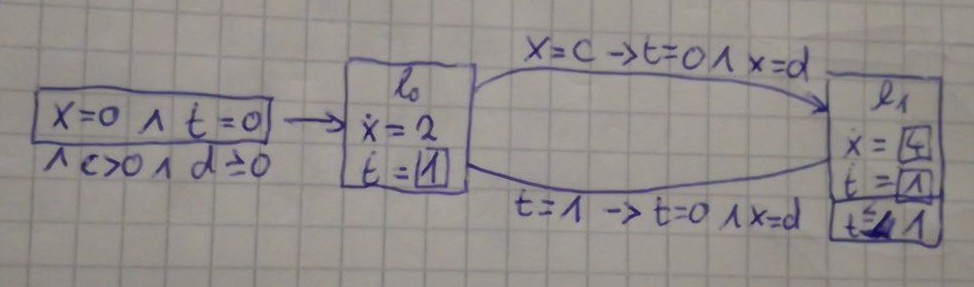
\includegraphics[width=\textwidth]{1.jpeg}

\subsection*{Aufgabenteil b:}

$\mathcal{H}$ = (Loc, Var, Lab, Edge, Act. Inv, Init)\\
\begin{itemize}
\item Loc = $\{l_0, l_1\}$
\item Var = \{x,t,c,d\}
\item Lab = $\emptyset$
\item Edge = \{($l_0$, $\emptyset$, x=c, t=0 $\wedge$ x=d, $l_1$), ($l_1$, $\emptyset$, t=1, t=0 $\wedge$ x=d, $l_0$)\}
\item Inv = \{($l_1$, $t\leq 1$)\}
\item Init = \{($l_0$, $x=0\wedge t=0\wedge c=0\wedge d=0$)\}
\end{itemize}